\documentclass[linenumbers,twocolumn]{aastex631}
% \documentclass[linenumbers]{aastex631}

% Packages
\usepackage[utf8]{inputenc}
\usepackage{graphicx}
\usepackage{amsmath}
\usepackage{amssymb}
\usepackage{enumitem}
\usepackage{ulem}
\usepackage{hyperref}

% Editing commands
\newcommand{\mm}[1]{{\textcolor{purple}{\bf #1}}}

% Make upright subscripts and superscripts in Mathmode.
\def\subinrm#1{\sb{\mathrm{#1}}}
{\catcode`\_=13 \global\let_=\subinrm}
\mathcode`_="8000
\def\supinrm#1{\sp{\mathrm{#1}}}
{\catcode`\^=13 \global\let^=\supinrm}
\mathcode`^="8000
\def\upsubscripts{\catcode`\_=12 } \def\normalsubscripts{\catcode`\_=8 }
\def\upsupscripts{\catcode`\^=12 } \def\normalsupscripts{\catcode`\^=7 }

\newcommand{\vdag}{(v)^\dagger}
\newcommand\aastex{AAS\TeX}
\newcommand\latex{La\TeX}

% Title
\shorttitle{Deriving the Shock Crossing Time}
\shortauthors{Moss M.} 

\begin{document}

\upsubscripts
\upsupscripts

\title{Deriving the Shell Crossing Time as a Function of the Density}

\correspondingauthor{Michael Moss}
\email{mikejmoss3@gmail.com}

\begin{abstract}
The goal of this derivation to estimate the time it will take a reverse shock to cross incoming ejecta material.

\end{abstract}

\section{Introduction}
{
    In the refreshed shock model, the wind of a GRB can be separated into two regions, (i) early outflow launched with $\bar{\Gamma}\sim150$ and (ii) later ejecta launched launched with $\bar{\Gamma}\sim15$. The early material is responsible for producing the prompt emission and the afterglow continuum emission. The later ejecta will eventually catch up to the early ejecta as it sweeps up circumburst medium and decelerates. When the later ejecta catches up and collides with the early material, a ``refreshed'' shock occurs, injecting energy into the front of the outflow and may be witnessed as bumps in the afterglow light curves (potentially in the optical regime). In this work, we would like to estimate the time it takes the incoming energy injected from the later ejecta to be distributed across the newly shocked material. This timescale should be dominated by the shell crossing time $t_{\Delta }$, where we model the incoming late ejecta as a shell with width $\Delta$, density $n_4$, and Lorentz factor $\gamma_{4}\sim15$ (see Figure \ref{fig: schematic} for a schematic). 

    To estimate $t_{\Delta}$, we must estimate the density of the rapid material ($n_4$) and the material which the late ejecta is colliding with ($n_1$). 
}

\section{Estimating Density of Zone 1 Material}
{
    The average particle density of the outflow material $n_{ej}$ (fluid frame) can be approximated as,

    \begin{align}
    n_{ej}(t) &= \frac{E_{iso}\Gamma(t)}{4\pi m_p c^2 \Gamma_0 R(t)^3} \label{eq: dens estim}
    \end{align}

    where $R(t)$ is the distance of the material from the central engine, $E_{iso}$ is the isotropic equivalent energy, $\Gamma_0$ is the initial bulk Lorentz factor of the ejecta, and $\Gamma(t)$ is the bulk Lorentz factor as a function of time (all in the central engine frame).

    We can estimate this density using a fiducial values for the isotropic equivalent energy $\dot{E}_{iso} = 10^{52}$ erg/s and for the radius and Lorentz factor of the material, but as stated in the introduction, we are most likely in the situation where the Zone 1 material we are considering will be early ejecta that has already been crossed by the external forward shock. The location and associated Lorentz factor when this material is completely crossed by a forward shock is not known, as such I will use an upper and lower limit for both, $R=10^{15}$ ($10^{16}$) cm, and $\bar{\Gamma} = 150$ (50) which results in a density of $n_{ej,upr} \approx 5.3\times 10^{9}$ ($\approx 1.7\times 10^{6}$) cm$^{-3}$. This will be the approximate density of the early ejecta before being crossed by the external reverse shock.

    Now, we must find the density increase between the unshocked and shocked early ejecta. Following Sari and Piran 1995 (hereafter SP95), we will designated the density and Lorentz factor of the unshocked ejecta material as $n_{4,SP} = n_{ej}$ and $\gamma_{4,SP} \sim 150$, respectively. Likewise, the density and Lorentz factor of the material already crossed by the external reverse shock material is noted as $n_{3,SP}$ (fluid frame), which can be approximated as

    \begin{align}
        n_{3,SP} &= n_{4,SP}\bigg(2\bigg[\sqrt{2\gamma_{4,SP}} \left(\frac{n_{1,SP}}{n_{4,SP}}\right)^{1/4}+\nonumber\\ 
        & \sqrt{\frac{1}{2\gamma_{4,SP}}} \left(\frac{n_{4,SP}}{n_{1,SP}}\right)^{1/4} \bigg] + 3\bigg)
    \end{align}

    Where $n_{1,SP} \sim 1 $ cm$^{-3}$ is the circumburst density and leads to an estimate of $n_{3,SP} \sim 2\times10^{11}$ ($\sim 2\times10^{7}$) cm$^{-3}$. This is very uncertain and most likely a large underestimation of the true density in the shocked material.
}

\section{Estimating the Shell Crossing Time}
{
    We can describe the width of the incoming late ejecta shell with respect to the density of the material, 

    \begin{align}
        \Delta &= \frac{E_{late,iso}}{4 \pi m_p c^2 \gamma_4^2 R^2 n_4} \label{eq: delta}
    \end{align}

    where $E_{iso,late}\sim10^{52}$ erg is the isotropic equivalent energy of the late material. Following SP95, the time it takes an incoming relativistic shell to be crossed by a reverse shock is given by the expression, 

    \begin{align}
        t_{\Delta} = \frac{\Delta}{c(\beta_4 - \beta_2)} \left(1-\frac{\gamma_4 n_4}{\gamma_3 n_3}\right)
    \end{align} 

    where $\beta_i = \sqrt{1 - 1/\gamma_i^2}$.

    The shell crossing time depends on the density ratio $f = n_4/n_1$, where in this scenario $n_1 = n_{3,SP}$ found earlier. If $\gamma_4^2 \gg f$, the we are in a relativistic regime and the shell crossing time can be expressed as 

    \begin{align}
        t_{\Delta} = \Delta \gamma_4 \frac{\sqrt{f}}{2c}
    \end{align}

    Note, in this formalism, if $n_4> 2 n_1 / \gamma_4$, then the shock crosses the shell faster than the speed of light. 

    If $f\gg\gamma_4^2$, then the reverse shock is in a Newtonian regime and the shell crossing time is expressed as

    \begin{align}
        t_{\Delta} = \sqrt{\frac{9}{14}}\Delta\gamma_4\frac{\sqrt{f}}{c}
    \end{align}

    The shell width and shell crossing time are displayed as a function of the late ejecta density in Figure \ref{fig: shell width} and \ref{fig: shell cross time}, respectively. 

    \begin{figure}[t!]
        \centering
        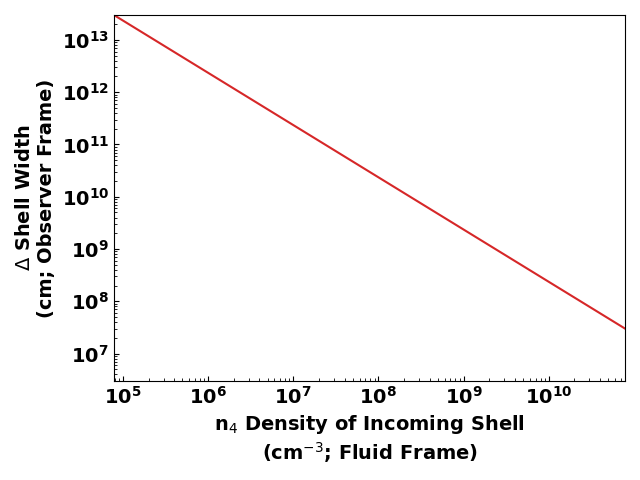
\includegraphics[width=0.45\textwidth]{shell-width.png}
        \caption{Late ejecta shell width $\Delta$ as a function of the density of the material (see Equation \ref{eq: delta}) }
        \label{fig: shell width}
    \end{figure}

    \begin{figure}[t!]
        \centering
        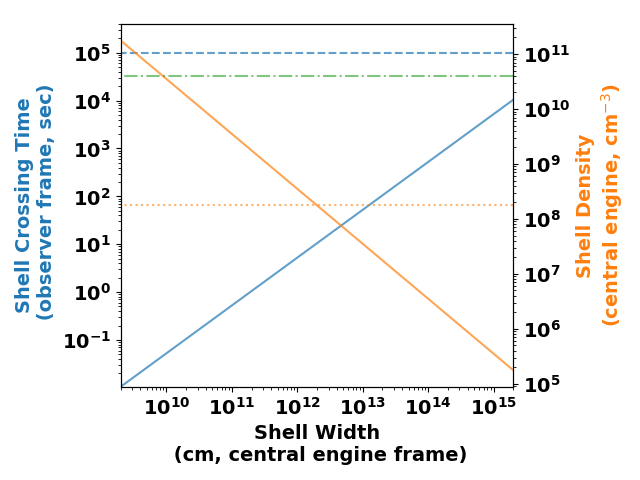
\includegraphics[width=0.45\textwidth]{shell-cross-time.png}
        \caption{Shell crossing time as a function of the density of the late ejecta material responsible for the refreshed shocks. The estimated density (which is likely an underestimate) is shown by the orange, dashed line and is estimated as $n_4 \sim 7.8 \times 10^{6}$ cm$^{-3}$. The green line indicates $10^{5}$ seconds, which is the approximate rise time of the bumps in optical afterglow of GRB030329.}
        \label{fig: shell cross time}
    \end{figure}
}

    \begin{figure*}[t!]
        \centering
        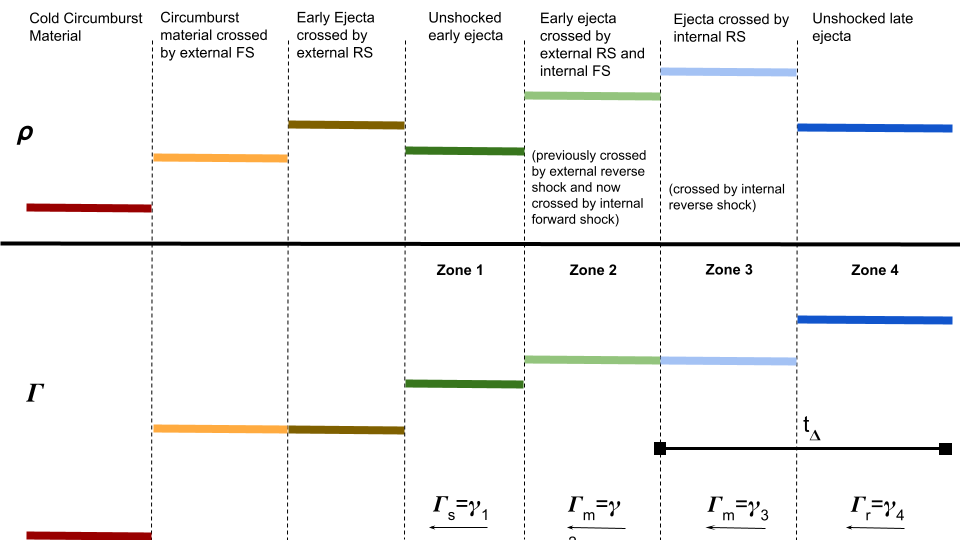
\includegraphics[width=0.7\textwidth]{schematic-pre-rs-complete.png}\\
        \vspace{1cm}
        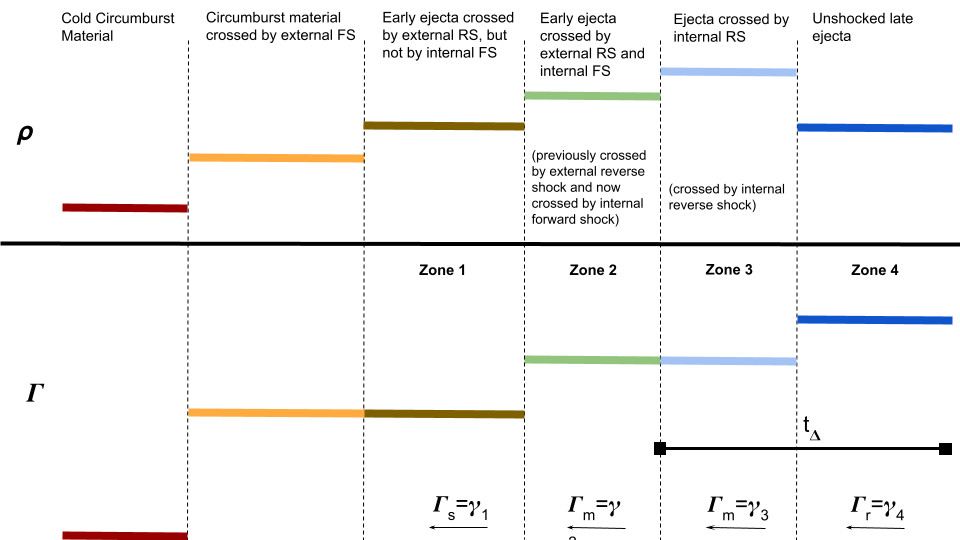
\includegraphics[width=0.7\textwidth]{schematic-aft-rs-complete.png}
        \caption{Schematic of the scenario (in the central engine frame). There are two ``reverse shocks'' in question, the reverse shock arising from the bulk of the jet decelerating as it sweeps up circumburst medium, which will be referred to as the external reverse shock, and an internal reverse shock arising from the deceleration of the incoming later ejecta decelerating as it rams the material in front of it (which happens to be the material previously crossed by the external reverse shock). The top panel shows a the situation we encounter if the late ejecta catches up to early material before the external reverse shock completely crosses the early material. It is more common that we will be in the case where the late material is colliding with early that has already been completely crossed by the external reverse shock (bottom panel).}
        \label{fig: schematic}
    \end{figure*}

\end{document}
